% C2GES original-title reconstruction, Round 3.
% Scientific evidence: independently audited v0.3.1 post-audit corrective run only.
\documentclass[applsci,article,submit,moreauthors]{Definitions/mdpi}
\firstpage{1}
\makeatletter\setcounter{page}{\@firstpage}\makeatother
\pubvolume{1}\issuenum{1}\articlenumber{0}\pubyear{2026}\copyrightyear{2026}
\datereceived{}\daterevised{}\dateaccepted{}\datepublished{}
\newcommand{\cges}{C\textsuperscript{2}GES}
\setlength{\headheight}{20pt}
\AtBeginDocument{\pdfstringdefDisableCommands{\def\cges{C2GES}}}

\Title{Causal and Counterfactual Graph-Enhanced Extractive Summarization (C\texorpdfstring{\textsuperscript{2}}{2}GES) for Power Grid Maintenance Reports}
\Author{Liu Bijing $^{1,2}$ and Yang Yong $^{1,2,}$*}
\AuthorNames{Liu Bijing and Yang Yong}
\address{$^{1}$ \quad NARI Group Corporation (State Grid Electric Power Research Institute), Nanjing 211106, Jiangsu Province, China;\\
$^{2}$ \quad Beijing Kedong Electric Power Control System Co., Ltd., Beijing 100080, China}
\corres{Correspondence: Yang Yong; liubijing@outlook.com}

\abstract{The title states an aspirational application to power-grid maintenance reports; the evaluated population is a selected public NERC technical-report proxy corpus, so maintenance transfer remains untested. We present \cges{}, a deterministic extractive framework combining centroid relevance, lexical role evidence, a typed textual proxy graph, and node-deletion path utility; the graph does not identify physical causal effects. Conservative gates retained 27 of 40 complete PDFs: 12 development and 15 test reports, yielding 12,924 non-summary candidates. In one authorized corrective run, Full \cges{} achieved Executive-Summary ROUGE-L F1 of 0.1060 at five sentences and 0.1276 at ten. It exceeded Semantic-MMR and TextRank on this split, but under equal sentence counts Full averaged 103.0/214.5 and 110.7/199.9 more words, respectively; these are not length-controlled advantages. Full was below the strict no-counterfactual graph ablation by about 0.0033 at both budgets, with intervals crossing zero. A post-unblinding development-only search of 147 configurations selected zero counterfactual weight in all 12 leave-one-report-out folds. The path mechanism is therefore an auditable structural diagnostic, not a demonstrated ROUGE-improving component. ROUGE measures lexical overlap, not quality, safety, or utility.}
\keyword{extractive summarization; typed textual proxy graph; structural perturbation; power-grid reports; NERC; reproducible evaluation}
\featuredapplication{Aspirationally, the framework could support source-linked navigation of maintenance reports. The present evidence is limited to a NERC technical-report proxy corpus. The output is not for operational decisions or autonomous root-cause analysis; engineers must inspect the source, and unsafe omissions remain unevaluated.}

\begin{document}

\section{Introduction}

Power-grid reliability and maintenance review requires more than retrieving isolated high-frequency terms. Engineers may need the sequence linking a condition or root cause to an initiating event, propagation or response, impact, and mitigation. Extractive summarization is attractive because each selected sentence can retain a stable source identifier from which a page locator can be recovered. It also exposes a difficult trade-off: sentences that are individually relevant may not preserve a coherent technical chain.

Evidence selection, query-focused summarization, and graph ranking provide foundations for sentence-level selection \cite{thorne2018fever,zhong2021qmsum,vig2022exploring,wang2020heterogeneous}. Dense sentence encoders offer strong semantic ranking comparators \cite{reimers2019sentencebert}, whereas causal NLP emphasizes that association and text-derived direction should not be confused with identified causal effects \cite{feder2022causal,du2022ecare}. These distinctions matter in critical-infrastructure text.

The exact title retains continuity with the original research objective, but ``for Power Grid Maintenance Reports'' denotes an aspirational intended downstream use rather than the population evaluated here. The empirical corpus comprises public NERC reliability, disturbance, event-analysis, recommendation, and assessment reports \cite{nercEventAnalysis,nerc2015qualityreport}; it contains maintenance-relevant lessons and corrective actions but not utility work orders, inspection records, or field-maintenance narratives. Every empirical statement below therefore concerns the selected NERC technical-report proxy corpus. Effectiveness, safety, and usefulness on title-concordant maintenance records remain untested.

An earlier implementation used fixed excerpts, allowed Executive Summary leakage, and defined a deletion quantity algebraically equivalent to weighted degree. Those v0.1/v0.2 results are withdrawn from the scientific claims of this article. The corrective rebuild uses complete PDFs and defines ``counterfactual'' narrowly as a computational graph perturbation: remove one sentence node and recompute registered typed-path utility. This operation neither generates alternative events nor estimates what the grid would have done under an intervention.

The contributions are fourfold. First, we construct a full-PDF corrective benchmark with explicit inclusion, extraction, leakage, split, and rights ledgers. Second, we define an auditable typed-path structural diagnostic whose node-deletion score is not reducible to weighted degree; no physical causal identification is claimed. Third, we compare seven conditions at two budgets using report-level paired estimates, a strict single-channel ablation, and a post-run exact sign-flip sensitivity. Fourth, we preserve the unfavorable counterfactual ablation, the completed zero-weight development calibration, and the maintenance-transfer boundary instead of converting them into favorable performance claims.

\section{Related Work}

\subsection{Extractive Technical-Document Summarization}

Extractive methods retain source text and are therefore naturally auditable. Lead, centroid, and graph-ranking methods remain useful comparators because they reveal whether complex selectors add value over position or centrality \cite{zhong2020extractive,bi2021aredsum,liu2021unsupervised}. TextRank is a primary graph-ranking reference \cite{mihalcea2004textrank}. Long reports also require diversity control; relevance-only selection can repeat a local event while omitting consequences or mitigation. The present task is global report summarization: each method receives identical candidates from one report and returns five or ten sentences in source order.

\subsection{Graphs, Semantic Ranking, and Causal Language}

Graph summarizers model relations among sentences, entities, topics, or discourse units \cite{wang2020heterogeneous,cui2020enhancing,jing2021multiplex}. \cges{} instead uses an interpretable typed sentence graph, trading learned capacity for deterministic construction and auditability. Semantic-MMR supplies a stronger non-graph baseline by combining dense centroid relevance with pairwise diversity.

Causal language requires an explicit boundary. A text-derived directed edge can reflect rhetorical order, lexical overlap, or a heuristic role transition. It is not a validated structural equation or a physical power-system mechanism \cite{feder2022causal}. We therefore use ``causal'' for the intended role vocabulary and ``counterfactual'' for node-deletion structural sensitivity, while repeatedly identifying both as proxies.

\subsection{Power-Grid Text Analytics}

Language technologies have been considered for grid models, operational records, and infrastructure analysis \cite{xie2022massively,hamann2024foundation,madabhushi2023survey,srinivasan2023artificial}. Supervised entity--relation extraction from a grid-field corpus is related but does not solve report-level summarization \cite{meng2023gridfield}. Our study evaluates authentic public technical reports but does not claim validated maintenance-workflow utility.

\section{Materials and Methods}

\subsection{Task, Scope, and Evidence Class}

Let report $D=\{s_1,\ldots,s_n\}$ contain non-summary candidate sentences. For budget $K\in\{5,10\}$, method $m$ returns $\hat{Y}_{m,K}\subseteq D$, with $|\hat{Y}_{m,K}|=\min(K,n)$. The selected sentences are restored to source order. The official Executive Summary is the reference only and is never candidate input.

ROUGE-1, ROUGE-2, and ROUGE-L F1 quantify lexical overlap between the extract and that Executive Summary \cite{lin2004rouge}. We use ROUGE-L as the registered primary endpoint. In this design, ``better ROUGE'' means greater Executive-Summary lexical overlap; it is not synonymous with accuracy, factual sufficiency, causal-chain correctness, maintenance quality, safety, or operator usefulness.

This is a post-audit corrective evaluation. Earlier versions of the test population were inspected while diagnosing R1, so the v0.3.1 freeze cannot recover outcome-unseen confirmatory status. The formal output is therefore descriptive evidence for a fixed corrective benchmark. A new sealed holdout would be required for confirmation.

\subsection{Source PDFs, Inclusion, and Leakage Gates}

The manifest binds 40 complete local PDFs with distinct SHA-256 values and 3200 declared pages. A deterministic full-PDF builder retained 27 reports and excluded 13 before outcome computation. The retained data comprise 12 development and 15 test reports. Their complete, development, and test SHA-256 values are \texttt{87F7F754...AA15}, \texttt{27CE41D...7F79}, and \texttt{A9342BD...D127}. Figure~\ref{fig:data-flow} summarizes the construction.

Supplementary Table~S1 is the rights-safe sampling frame for all 40 reports. For every source it records a non-verbatim report identifier, genre, declared pages, reference word count where a valid reference was detected, candidate count, split or exclusion branch, reason, source-navigation locator, and permission status. The branch is exhaustive: 27 inclusion records and 13 exclusion records equal the 40-report inventory. Because redistribution rights were not established for the PDFs or extracted prose, neither is included in the transferable package. The metadata inventory supports audit and source navigation; it is not a substitute for permission.

\begin{figure}[H]
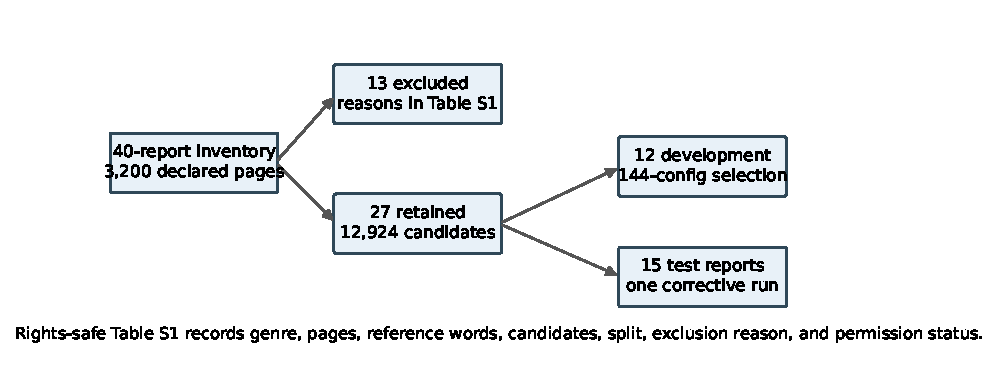
\includegraphics[width=\textwidth]{figures/fig02_dataset_flow.pdf}
\caption{Dataset construction and partitioning. Conservative boundary and quality gates retained 27 of 40 full PDFs. The 12-report development split was used for configuration selection; one authorized run evaluated the 15-report test split.}
\label{fig:data-flow}
\end{figure}

Candidates begin after a conservatively detected Executive Summary boundary, and no fixed sentence cap is applied. The builder emits 12,924 candidates, with 51--1898 per report; 25 reports have more than 80. An independent rebuild found zero reference/body page-interval overlap, zero normalized exact candidate/reference match, zero normalized common substring of at least 50 characters, and zero occurrences of eight registered extraction-pollution patterns. These checks address registered leakage and pollution modes but do not establish semantic cleanliness of every sentence.

\subsection{Sentence Roles and Typed Textual Proxy Graph}

Each candidate receives lexical evidence for root cause, trigger event, propagation or response, impact, and mitigation. Positive top-score ties abstain rather than using fixed role order; 111 development ties all received no dominant role and no incident directed edge. No silver role label is supplied to the v0.3 selector.

Table~\ref{tab:taxonomy} gives the executable taxonomy. The cues are substring-based lexical indicators, normalized within a report. A unique positive maximum assigns a dominant role; an all-zero vector or equal positive maximum yields abstention. The system does not detect grammatical scope, factual status, or document-level coreference.

\begin{table}[H]
\caption{Executable role and transition taxonomy. These are lexical text proxies, not expert labels or physical relations.}
\label{tab:taxonomy}\centering\small
\begin{tabularx}{\textwidth}{p{2.2cm}XX}
\toprule
Role & Representative registered cue classes & Permitted outgoing transitions\\
\midrule
Root cause & cause, due-to, failure, and protection-setting terms & trigger; propagation or response; mitigation\\
Trigger event & fault, outage, initiation, trip, and fire terms & propagation or response; impact\\
Propagation or response & trip, voltage, frequency, islanding, load-shed, reserve, and flow terms & impact\\
Impact & quantities with grid units, customer, load, loss, and unavailability terms & mitigation\\
Mitigation & recommendation, corrective, preventive, and standard terms & none\\
Abstention & no positive cue, or more than one equal positive maximum & none\\
\bottomrule
\end{tabularx}
\end{table}

A directed edge is allowed only for registered stage-monotone role transitions within 12 sentence positions. Its weight combines positional distance, token-set Jaccard overlap, and role confidence. Normalized weighted degree forms graph salience $G_i$. Figure~\ref{fig:algorithm} displays the executable flow and its claim boundary.

\begin{figure}[H]
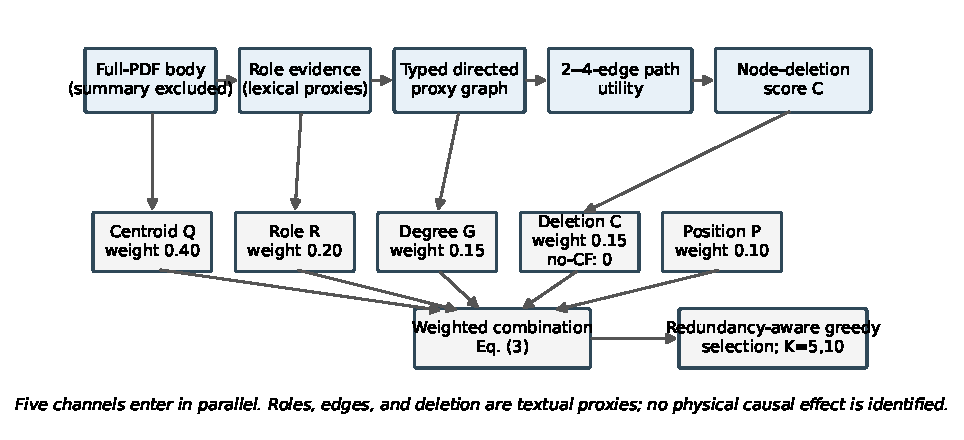
\includegraphics[width=\textwidth]{figures/fig01_algorithm.pdf}
\caption{Implemented \cges{} pipeline. The five channels $Q,R,G,C,P$ enter the weighted combination in parallel; strict no-CF sets only $C$ to zero before the same selector. Roles, edges, and node deletions are deterministic textual proxies, not a learned graph neural network, physical simulator, or causal identification.}
\label{fig:algorithm}
\end{figure}

\subsection{Typed Path-Deletion Structural Perturbation}

Let $\mathcal{P}(G)$ be the set of simple, stage-monotone paths with two to four edges beginning at a root-cause or trigger node and ending at an impact or mitigation node. For path $p$,
\begin{equation}
\operatorname{strength}(p)=\left(\prod_{e\in p}w_e\right)^{1/|p|}\frac{\max\operatorname{stage}(p)-\min\operatorname{stage}(p)}{4}.
\end{equation}
The graph utility and raw deletion score are
\begin{equation}
U(G)=\sum_{p\in\mathcal{P}(G)}\operatorname{strength}(p),\qquad
C_i=U(G)-U(G_{-i})=\sum_{p\ni i}\operatorname{strength}(p).
\end{equation}
Unlike weighted degree, $C_i$ depends on qualified multi-edge path membership, role order, and the geometric mean of edge weights. A registered counterexample gives two nodes equal weighted degree but unequal qualified-path membership. Unit tests verify deletion-loss equality, deterministic scaling, cache equivalence, and fail-closed work limits. These checks establish software and mathematical non-identity, not physical causality or effectiveness.

\subsection{Scoring and Selection}

The development-selected Full score is
\begin{equation}
S_i=0.40Q_i+0.20R_i+0.15G_i+0.15C_i+0.10P_i,
\end{equation}
where $Q_i$ is lexical centroid relevance, $R_i$ role evidence, $G_i$ weighted-degree salience, $C_i$ normalized path-deletion loss, and $P_i$ a positional prior. Greedy selection subtracts $0.50$ times the maximum token-set Jaccard overlap with an already selected sentence. Path and expansion caps are 250,000 and 2,000,000 and fail closed on exhaustion.

The strict no-CF ablation changes only the coefficient of $C_i$ from 0.15 to zero. It does not renormalize any remaining coefficient or alter candidates, graph construction, redundancy penalty, tie rules, or budgets. This single-factor contrast isolates the implemented perturbation channel.

The output is designed for source navigation rather than stand-alone decision support. The frozen prediction record preserves report ID and sentence ID; a deterministic, non-verbatim locator ledger joins those identifiers to page, source order, report metadata, and source URL using the protected candidate table. All 1,575 selected references resolved uniquely to an integer page within the declared PDF range. Thus, the page can be recovered through the locator ledger, but it was not emitted directly in the prediction JSONL. A reviewer can reopen the page, read the surrounding section, and inspect claims omitted from the extract. No output should be used for an operational decision without this source check. In particular, missing mitigations, qualifications, negation, or uncertainty can make a fluent extract unsafe.

\subsection{Known Linguistic Failure Modes}

No qualified experts supplied role or relation gold labels. Accordingly, Table~1 is a summary of executable behavior rather than validated semantic annotation; the exact lexicon, normalization, transitions, and tests are preserved in the packaged code snapshot, while the public repository remains unsynchronized. Ambiguous lexical ties abstain mechanically, but an unambiguous wrong cue can still assign a role. Negated statements (for example, a sentence saying that an outage did not occur) can activate an event cue because negation scope is not modeled. Hypothetical, conditional, quoted, or historical events can likewise receive factual-looking roles. A transition may connect lexically compatible sentences within 12 positions even when discourse context does not support the relation. These cases define an error taxonomy for future expert evaluation; they are not counts of verified errors in the present corpus.

\subsection{Development Selection and Comparators}

The 12-report development search evaluated 144 registered configurations. Its ordered objective maximized mean ROUGE-L F1 at $K=5$, then mean ROUGE-1 F1, lower redundancy, and earliest ledger position. Grid index 60 was selected, with mean development ROUGE-L F1 0.1195126 and ROUGE-1 F1 0.2713870. Full minus strict no-CF development ROUGE-L was $-0.0056652$; this negative result was retained before the formal test.

Seven frozen conditions share the same candidate space: Lead, lexical Centroid, TextRank, Semantic-MMR, Role, graph without CF (strict), and Full \cges{}. Semantic-MMR uses a frozen local all-MiniLM-L6-v2 snapshot and greedily maximizes $0.5\cos(e_i,\bar e_D)-0.5\max_{j\in A}\cos(e_i,e_j)$ \cite{reimers2019sentencebert}. Its symmetric coefficient was not optimized on development or test outcomes.

\subsection{Frozen Evaluation and Statistical Interpretation}

The v0.3.1 freeze registers ROUGE-L F1 as primary and three Full-minus-baseline contrasts (strict no-CF, Semantic-MMR, TextRank) at each budget. Paired report-level percentile bootstrap intervals use 10,000 resamples. For paired deltas $d_1,\ldots,d_{15}$, each resample draws 15 reports with replacement and yields mean $\bar d_b$. The registered tail quantity is
\begin{equation}
t_{\mathrm{boot}}=2\min\left\{B^{-1}\sum_{b=1}^{B}\mathbb{1}(\bar d_b\leq0),\;B^{-1}\sum_{b=1}^{B}\mathbb{1}(\bar d_b\geq0)\right\},\quad B=10{,}000.
\end{equation}
Because these resamples are centered on the observed deltas rather than generated under a null, $t_{\mathrm{boot}}$ is a descriptive bootstrap sign-tail estimator, not a calibrated hypothesis-test $p$ value. The frozen machine values and their registered Holm transformation are preserved as provenance, but no significance claim is based on them. ROUGE-1, ROUGE-2, redundancy, and other pairings are descriptive \cite{cameron2008bootstrap}.

After the run, without rerunning any model or changing a prediction, we added an unregistered exact paired sign-flip sensitivity. For each contrast, all $2^{15}=32{,}768$ report-level sign assignments were enumerated and the two-sided value was the proportion whose absolute mean was at least the observed absolute mean. This procedure assumes report-level independence and sign exchangeability (equivalently, symmetry of paired errors around zero under the null); it does not follow from the data and may be fragile for heterogeneous reports. Zero deltas remain invariant. The six exact values were adjusted as one family by Holm's step-down procedure \cite{holm1979simple}. This analysis is labelled post-run sensitivity rather than confirmatory inference. The freeze binds data, code, configuration, model tree, dependency lock, tests, and corrective history.

One authorized physical run produced 210 rows ($15\times7\times2$). Independent post-run audit rehashed 31 frozen files, recalculated all 28 aggregate values and all six contrast records with maximum absolute discrepancy zero, and returned PASS. The evidence class remains post-audit corrective descriptive.

\subsection{Post-Unblinding Development-Only Calibration}

After the v0.3.1 test result was revealed, a separate exploratory program evaluated 147 semantically deduplicated configurations using only the frozen 12-report development file (SHA-256 \texttt{27CE41D...7F79}). It varied counterfactual weight over seven values from 0 to 0.20, three weight-allocation rules, three path horizons, and three gating rules; duplicate settings were removed. Guards and the run manifest record \texttt{test\_input\_accessed=false} and \texttt{formal\_output\_accessed=false}. This chronology makes the analysis post-unblinding even though it did not read test artifacts.

Twelve leave-one-report-out development folds selected a zero-CF winner in 12/12 folds. The best nonzero candidate under the registered exploratory tie-break used weight 0.025, won 0/12 folds, and remained below strict zero-CF by 0.00131 at $K=5$ and 0.00091 at $K=10$; both development bootstrap intervals crossed zero. These findings do not replace v0.3.1 and were never evaluated on the revealed 15-report test set. They diagnose integration behavior and constrain future protocol design; they provide no confirmatory performance evidence.

\subsection{Generative-AI Assistance and Verification Boundary}

The OpenAI Codex agent interface was used to assist with prose drafting and editing, experiment and audit planning suggestions, Python and \LaTeX{} development and review, provenance-record preparation, and manuscript build and visual-quality checks. All numerical results reported in this article were obtained from the frozen experiment ledgers or from documented local code execution; Codex output was not used as a source of experimental measurements. No generative-AI system was treated as a qualified power-grid expert, human annotator, or adjudicator. All figures are code-native outputs generated locally from the packaged scripts and stated data sources. The authors reviewed the assisted work and retain responsibility for the study and manuscript.

\section{Results}

\subsection{Dataset and Execution Integrity}

Table~\ref{tab:audit} reports the principal audit quantities. Candidate page boundaries remained strictly after reference-summary pages for all 15 test reports, and every selected sentence ID/text pair matched its frozen source candidate.

\begin{table}[H]
\caption{Dataset and execution audit; the formal paired evaluation unit is the test report ($n=15$).}
\label{tab:audit}\centering
\begin{tabular}{lr}
\toprule
Item & Audited value\\
\midrule
Source PDFs / declared pages & 40 / 3200\\
Included / excluded reports & 27 / 13\\
Development / test reports & 12 / 15\\
Candidate sentences & 12,924\\
Reference/body page overlaps & 0\\
Exact normalized reference/candidate matches & 0\\
Common substrings $\geq50$ characters & 0\\
Prediction rows / expected rows & 210 / 210\\
Frozen-file hash checks at execution & 77 / 77 passed\\
Independent current rehashes & 31 / 31 passed\\
\bottomrule
\end{tabular}
\end{table}

\subsection{Aggregate Test Results}

Table~\ref{tab:all-results} contains all seven conditions and four recorded metrics at both budgets. Full \cges{} exceeded Semantic-MMR and TextRank on mean ROUGE-L at each equal-sentence budget but was below strict no-CF. Because extraction-unit lengths differ materially, these comparisons are not word- or token-budget controlled. Figure~\ref{fig:aggregate} visualizes the same ROUGE-L means and does not add a statistical test.

\begin{table}[H]
\caption{Macro-mean results over $n=15$ test reports at equal sentence counts, not equal word counts. Bold marks only the observed maximum ROUGE-L within a budget; underlining marks the minimum redundancy. Neither convention is an inferential conclusion.}
\label{tab:all-results}\centering\small
\begin{tabular}{llrrrr}
\toprule
$K$ & Condition & R-1 F1 & R-2 F1 & R-L F1 & Redundancy\\
\midrule
5 & Lead & 0.1633 & 0.0545 & 0.0878 & 0.0668\\
5 & Centroid & 0.1955 & 0.0457 & 0.0939 & 0.2333\\
5 & TextRank & 0.1508 & 0.0356 & 0.0806 & 0.2560\\
5 & Semantic-MMR & 0.1783 & 0.0433 & 0.0853 & \underline{0.0237}\\
5 & Role & 0.1889 & 0.0557 & 0.0934 & 0.0862\\
5 & Graph no-CF & 0.2497 & 0.0648 & \textbf{0.1094} & 0.0798\\
5 & Full \cges{} & 0.2359 & 0.0611 & 0.1060 & 0.0745\\
\midrule
10 & Lead & 0.2617 & 0.0811 & 0.1158 & 0.0554\\
10 & Centroid & 0.2809 & 0.0683 & 0.1196 & 0.2011\\
10 & TextRank & 0.2470 & 0.0615 & 0.1156 & 0.2149\\
10 & Semantic-MMR & 0.2840 & 0.0728 & 0.1133 & \underline{0.0269}\\
10 & Role & 0.3132 & 0.0848 & 0.1257 & 0.0550\\
10 & Graph no-CF & 0.3471 & 0.0930 & \textbf{0.1310} & 0.0746\\
10 & Full \cges{} & 0.3366 & 0.0874 & 0.1276 & 0.0667\\
\bottomrule
\end{tabular}
\end{table}

\begin{figure}[H]
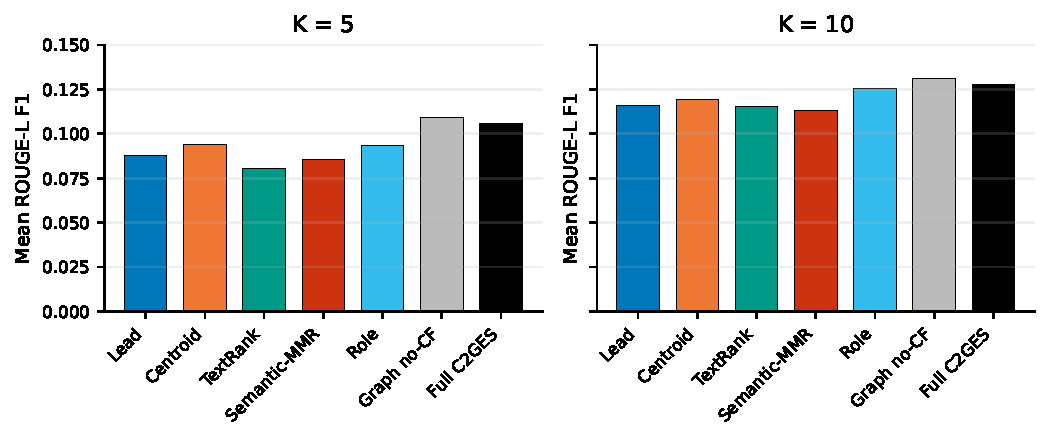
\includegraphics[width=\textwidth]{figures/fig03_aggregate_rougel.pdf}
\caption{Mean Executive-Summary ROUGE-L F1 for the seven frozen conditions ($n=15$ reports) at equal sentence counts but unequal word counts. Bars are descriptive macro-means; paired distributions and sensitivity results appear in Figure~\ref{fig:paired} and Tables~\ref{tab:contrasts}--\ref{tab:signflip}.}
\label{fig:aggregate}
\end{figure}

\subsection{Post-Run Output-Length and Extraction-Unit Diagnostics}

Without rerunning selection or changing any prediction, a hash-pinned script counted Unicode whitespace-delimited words and Unicode characters in every selected unit of the immutable ledger. Supplementary Table~S2 contains all 14 condition--budget groups and per-report records. Table~\ref{tab:length-audit} shows the four conditions used in the headline interpretation. The displayed long-unit and Table-marker counts are selection instances, so a unit selected by more than one condition or budget is counted in each corresponding output.

\begin{table}[H]
\caption{Post-run descriptive output-length diagnostics. ``$>100$'' counts selected-unit instances longer than 100 words; ``Table'' counts units containing the exact case-sensitive string. These quantities do not alter the frozen experiment.}
\label{tab:length-audit}\centering\small
\begin{tabular}{llrrrrr}
\toprule
$K$ & Condition & Mean words & Mean characters & $>100$ & Table & Maximum words\\
\midrule
5 & Full \cges{} & 287.7 & 1843.6 & 12 & 14 & 140\\
5 & Graph no-CF & 329.0 & 2099.9 & 15 & 16 & 270\\
5 & Semantic-MMR & 184.7 & 1242.1 & 5 & 9 & 138\\
5 & TextRank & 177.0 & 1125.1 & 1 & 7 & 124\\
10 & Full \cges{} & 568.9 & 3619.5 & 25 & 26 & 270\\
10 & Graph no-CF & 596.9 & 3822.5 & 28 & 26 & 270\\
10 & Semantic-MMR & 354.5 & 2361.2 & 7 & 16 & 138\\
10 & TextRank & 369.0 & 2329.7 & 4 & 18 & 130\\
\bottomrule
\end{tabular}
\end{table}

Full averaged 103.0 and 214.5 more words than Semantic-MMR at $K=5$ and $K=10$, and 110.7 and 199.9 more than TextRank. Among its 225 selected-unit instances, 37 exceeded 100 words, 40 contained ``Table'', and the maximum was 270 words. These diagnostics reveal fused table, heading, footnote, or line-break blocks in the sentence-level extraction units. Consequently, the observed ROUGE advantages over Semantic-MMR and TextRank are equal-sentence but unequal-word comparisons and do not establish fair length-matched superiority. Constructing newly selected word-budget systems on the revealed test would be a new post hoc experiment and was not done.

\subsection{Registered Contrasts}

Table~\ref{tab:contrasts} gives the six registered contrasts. Full minus strict no-CF was $-0.003332$ at $K=5$ and $-0.003360$ at $K=10$; both intervals crossed zero. Thus, neither development nor test evidence supports a lexical-overlap benefit from the counterfactual channel.

Full exceeded Semantic-MMR and TextRank at both equal-sentence budgets on this split, but the output-length audit shows that Full used substantially more words; no length-controlled superiority is claimed. The two registered machine sign-tail values stored as 0.0 mean only that zero smaller-tail draws occurred among 10,000 observed-delta bootstrap resamples. They are shown as ``0/10,000 tail draws,'' not as probabilities of zero or conventional $p$ values. The immutable machine artifact retains its original numeric values.

\begin{table}[H]
\caption{Registered Full-minus-baseline Executive-Summary ROUGE-L contrasts, paired by test report ($n=15$). The final column is the registered descriptive sign-tail estimator, not a calibrated $p$ value.}
\label{tab:contrasts}\centering\small
\begin{tabular}{llrrr}
\toprule
$K$ & Baseline & Mean difference & 95\% bootstrap CI & Registered $t_{boot}$\\
\midrule
5 & Graph no-CF strict & -0.003332 & [-0.010889, 0.002826] & 0.3544\\
5 & Semantic-MMR & 0.020737 & [0.012765, 0.028354] & 0/10,000 tail draws\\
5 & TextRank & 0.025438 & [0.017542, 0.033722] & 0/10,000 tail draws\\
10 & Graph no-CF strict & -0.003360 & [-0.008306, 0.001040] & 0.1444\\
10 & Semantic-MMR & 0.014360 & [0.006082, 0.022215] & 0.0008\\
10 & TextRank & 0.012029 & [0.004397, 0.019241] & 0.0022\\
\bottomrule
\end{tabular}
\end{table}

Table~\ref{tab:signflip} reports the unregistered post-run sensitivity. The exact values preserve the qualitative conclusion: the no-CF contrasts do not provide evidence of a positive counterfactual contribution, whereas the observed differences versus Semantic-MMR and TextRank are directionally stable under the stated sign-exchangeability assumption. Because the corpus is selected and $n=15$, this does not establish population-wide superiority.

\begin{table}[H]
\caption{Unregistered exact paired sign-flip sensitivity from the immutable prediction ledger ($n=15$, $2^{15}=32{,}768$ assignments per contrast). Holm adjustment covers all six values.}
\label{tab:signflip}\centering\small
\begin{tabular}{llrrr}
\toprule
$K$ & Baseline & Signs $+/-/0$ & Exact two-sided $p$ & Holm-adjusted $p$\\
\midrule
5 & Graph no-CF strict & 7/7/1 & 0.436768 & 0.436768\\
5 & Semantic-MMR & 14/1/0 & 0.000305 & 0.001526\\
5 & TextRank & 14/1/0 & 0.000122 & 0.000732\\
10 & Graph no-CF strict & 6/8/1 & 0.200684 & 0.401367\\
10 & Semantic-MMR & 11/4/0 & 0.006592 & 0.026367\\
10 & TextRank & 13/2/0 & 0.009644 & 0.028931\\
\bottomrule
\end{tabular}
\end{table}

Figure~\ref{fig:paired} exposes every report-level difference. Full and strict no-CF selected different sentence sequences in 28 of 30 report--budget cells, and their base scores differed in all 30, confirming an active but not beneficial channel.

\begin{figure}[H]
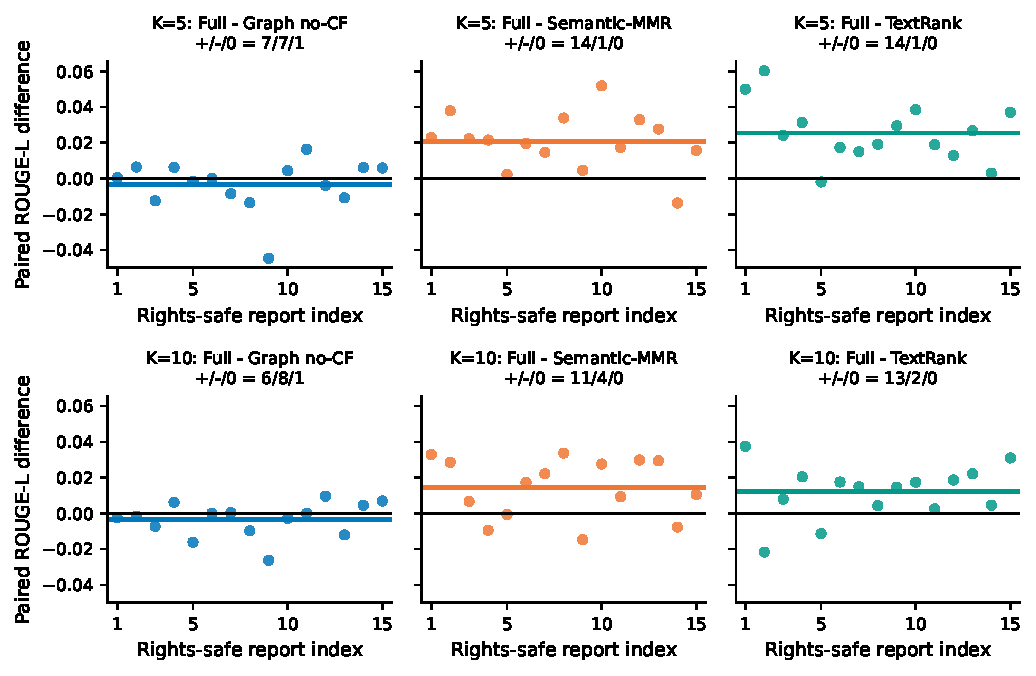
\includegraphics[width=\textwidth]{figures/fig04_paired_differences.pdf}
\caption{Per-report paired Executive-Summary ROUGE-L differences for the six registered contrasts ($n=15$). Horizontal colored segments denote means; black lines denote zero; panel titles give positive/negative/zero sign counts. Rights-safe report indices map to non-verbatim metadata in Supplementary Table~S1.}
\label{fig:paired}
\end{figure}

\subsection{Computational Diagnostics}

Across 19,008 Full/no-CF sentence-score comparisons, 9774 were nonzero and the maximum absolute difference was 0.15. Maximum observed path expansions were 19,638 of the 2,000,000 cap, and maximum qualifying paths were 16,182 of 250,000; no fail-closed path limit was approached. These diagnostics confirm that the mechanism executed as specified, but do not convert it into a useful ranking component.

\subsection{Exploratory Development Calibration Result}

The post-unblinding development-only calibration did not find a defensible nonzero counterfactual coefficient. Candidate C046, with zero counterfactual weight, won every one of the 12 leave-one-report-out folds. The best nonzero candidate, C055 with weight 0.025, won no fold and remained slightly below its strict-zero comparison at both budgets. The original frozen 0.15-weight development configuration was below strict zero by 0.00567 at $K=5$ and 0.00257 at $K=10$. These development findings are reported because they followed disclosure of the formal result; they cannot replace, tune, or reinterpret the immutable v0.3.1 test.

\section{Discussion}

\subsection{Supported Interpretation}

The rebuild establishes a cleaner experimental object than R1: complete-PDF candidates, multi-level summary-leakage checks, a recorded development search, a path-based score distinct from degree, a Semantic-MMR baseline, and report-level paired estimates. Full \cges{} had higher mean Executive-Summary ROUGE-L than Semantic-MMR and TextRank on this retained split, but used markedly more words at both equal-sentence budgets. The unregistered exact sign-flip sensitivity retained the ROUGE directions after six-value Holm adjustment under a stated sign-exchangeability assumption; it does not control output length or turn the corrective split into confirmatory evidence.

System-level baseline differences should not be attributed to the named counterfactual mechanism. Strict no-CF produced the highest observed ROUGE-1, ROUGE-2, and ROUGE-L at both budgets, while the Full-minus-no-CF intervals crossed zero. The proper conclusion is that path deletion is an identifiable structural feature whose incremental lexical-overlap value was not demonstrated.

\subsection{Causal and Counterfactual Boundaries}

The graph organizes text into role-conditioned paths. Direction and path score are reproducible hypotheses, not validated relations in grid physics. Node deletion measures the dependence of graph utility on one sentence; it is not a potential-outcome estimand, a do-intervention on grid state, or evidence that an event would change if a sentence were absent. The title must therefore be read together with these boundaries.

\subsection{Maintenance-Workflow Transfer}

NERC reliability and disturbance reports can inform maintenance-oriented lessons-learned review, but work orders and inspection records differ in vocabulary, length, asset granularity, narrative structure, and reference-summary availability. Current evidence measures Executive-Summary lexical overlap on a selected NERC technical-report proxy corpus and motivates, but does not validate, a maintenance-review use case. It does not establish effectiveness for operational maintenance reports.

\subsection{Limitations}

The test set contains only 15 selected public reports from one organization and derives from a population inspected during corrective reconstruction. Official Executive Summaries are long references, and ROUGE/redundancy do not measure factual sufficiency, engineering usefulness, unsafe omission, or causal-chain correctness. Equal sentence counts yielded unequal word budgets, and fused table, heading, footnote, or line-break blocks occurred among extraction units; therefore current baseline advantages are not length controlled. Semantic-MMR used a fixed coefficient of 0.5 whereas \cges{} received a 144-configuration development search, so comparator tuning budgets were asymmetric. Role and edge construction lack blinded qualified-expert validation, and the ambiguity/negation/hypothetical taxonomy has no expert-gold error counts. Third-party rights restrict redistribution of PDFs and verbatim extracted text. The public repository has not yet been asserted to match the exact final-candidate package.

Post hoc tuning after seeing these results cannot rehabilitate the current test as confirmatory. The completed 147-configuration development-only calibration selected zero CF in all 12 folds and did not support its best nonzero setting. It did not access test input or formal output files, does not replace v0.3.1, and must not be evaluated on the revealed 15 reports. Any redesigned integration requires a new, genuinely unseen holdout.

\subsection{Future Validation}

Future work should freeze a license-cleared corpus of work orders or maintenance narratives at report or site level and create an untouched external holdout. Qualified power-grid personnel should independently score source faithfulness, coverage of cause/event/impact/mitigation, engineering usefulness, and unsafe omissions; disagreement and adjudication should be retained, and inter-rater agreement reported. LLM judgments may support annotation workflow experiments but must not be labeled expert validation.

\section{Conclusions}

\cges{} is rebuilt as a deterministic, auditable extractive method evaluated on full NERC technical reports. The exact title names an aspirational maintenance application, not a validated population. The typed path-deletion score is mathematically distinct from weighted degree, the benchmark has explicit leakage and extraction audits, and the comparison includes Semantic-MMR and a strict single-channel ablation. Full achieved Executive-Summary ROUGE-L F1 of 0.1060 and 0.1276 at five and ten sentences and had higher values than Semantic-MMR and TextRank on this retained split; however, it averaged 103.0/214.5 and 110.7/199.9 more words, respectively, so no length-controlled superiority is claimed. Full was lower than strict no-CF by approximately 0.0033 at both budgets, with intervals crossing zero, and post-unblinding development calibration selected zero CF in 12/12 folds. The study therefore supports an auditable structural diagnostic and bounded lexical-overlap comparisons, but not a counterfactual-component gain, real-world causal identification, summary safety, or maintenance-work-order effectiveness. The extracts are for source navigation, not operational decisions. Confirmation requires a new sealed, title-concordant holdout and qualified human validation.

\supplementary{The final-candidate manifest separates transferable non-verbatim material from a restricted-local compartment. The transferable set contains the 40-report rights-safe inventory; six exact sign-flip records; complete post-unblinding calibration code, 10 tests, verifier, state, four ledgers, decision, run manifest, audit, and three core code snapshots; output-length records for all 14 condition--budget groups; the 1,575-row non-verbatim page-locator ledger; configuration/freeze/authorization/dependency and independent-audit records; code-native figures with per-artifact lineage; and a 23-item citation-context audit. The restricted-local compartment binds the immutable 210-row prediction ledger because it contains verbatim derived text; it is excluded from the safe editor ZIP unless third-party permission is confirmed. Source PDFs and full extracted datasets are never packaged. Required-role, forbidden-file, exact-set, byte, and SHA-256 checks are machine verified.}
\authorcontributions{Conceptualization, B.L. and Y.Y.; methodology, B.L.; software, B.L.; validation, B.L.; formal analysis, B.L.; investigation, B.L.; resources, Y.Y.; data curation, B.L.; writing---original draft preparation, B.L.; writing---review and editing, B.L. and Y.Y.; visualization, B.L.; supervision, Y.Y.; project administration, Y.Y.; funding acquisition, Y.Y. All authors have read and agreed to the published version of the manuscript.}
\funding{This research was funded by the Science and Technology Research Project of State Grid Fujian Electric Power Co., Ltd., grant number 521300250006. The funder had no role in the design of the study; in the collection, analyses, or interpretation of data; in the writing of the manuscript; or in the decision to publish the results.}
\institutionalreview{Not applicable. This computational study uses published technical reports and does not involve human participants or animals.}
\informedconsent{Not applicable.}
\dataavailability{Code is intended for release at \url{https://github.com/gaoxingkele/c2ges}. The repository must be synchronized, licensed, tagged, archived, and verified from a fresh clone before submission; this final candidate does not assert that its current public contents reproduce the reported artifacts. Owing to third-party licensing restrictions, source PDFs and verbatim derived text are not publicly redistributed. Subject to applicable permissions, restricted materials needed for editorial and peer-review verification may be requested from the corresponding author. Rights-safe metadata, hashes, configurations, the non-verbatim selected-ID-to-page locator, descriptive diagnostic records, and reproducibility records accompany the manuscript-bound package.}
\acknowledgments{The OpenAI Codex agent interface was used for the generative-AI-assisted activities described in Materials and Methods. The exact backend model identifier and version were not retained in the project records. The authors reviewed the outputs and retain responsibility for the manuscript; Codex was not treated as an author, qualified power-grid expert, human annotator, or adjudicator.}
\conflictsofinterest{The authors declare no conflicts of interest.}

\begin{adjustwidth}{-\extralength}{0cm}
\reftitle{References}
\bibliography{references_cited_verified}
\PublishersNote{}
\end{adjustwidth}
\end{document}
